\section{Illuminazione}

 \'{E} ampiamente riconosciuto che l'appropriatezza
dell'illuminazione e la qualità della stessa siano aspetti critici nella
creazione di un sistema di visione pronto e robusto. Progettare un ambiente di
analisi robusto massimizzerà la riuscita del progetto in termini di tempo,
sforzo e risorse impiegate.

Storicamente, la luce è stato sempre l'ultimo aspetto ad essere specificato,
sviluppato o finaziato, questo tipo di approccio derivava principalmente
dall'assenza di prodotti commerciali espressamente rivolti alla machine
vision, ciò portava all'adozioni di prodotti consumer quali lampade a
incandescenza e/o fluorescenza.

Ciò che è realmente richiesto per la realizzazione di sistemi di ispezione
industriale è il controllo dell' illuminazione volto a produrre:

\begin{itemize}
	\item Illuminazione appropriata dei campioni da analizzare;
	\item Standardizzazione delle componenti, tecniche, implementazioni e dell'utilizzo del sistema di illuminazione;
	\item Riproducibilità dei risultati delle ispezioni;
	\item Robustezza delle ispezioni a variazioni dell'ambiente di ispezione;
\end{itemize} 

\subsection{Illuminazione direzionale}

Un illuminatore direzionale è costituito da una o più 
sorgenti di luce puntiforme che proiettano luce direzionale 
sulla parte da ispezionare, utilizzando questa tipologia di 
illuminatore è possibile ispezionare superfici piane non 
riflettenti poichè la luce raggiunge il sensore in maniera consistente. 

\begin{figure}
\centering
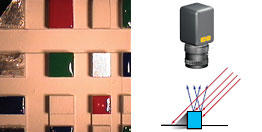
\includegraphics[width=.3\textwidth]{img/illuminazione-direzionale.jpg}
\caption{Illuminazione direzionale}\label{fig:illuminazione-direzionale}
\end{figure}

\begin{centering}
\centering
\begin{tabular}{l l}
Pro: &  Luminosità, flessibilità di installazione. \\
Contro: &  Generazione di ombre e riflessi dovuti ad altri oggetti presenti sulla scena \\
\end{tabular}
\end{centering}


\subsection{Illuminazione tangenziale}

Un illuminatore tangenziale è costituito da una o più 
sorgente di luce direzionale aventi un elevato angolo di 
incidenza rispetto alla parte da ispezionare, ciò li rende 
adatti ad evidenziare difetti superficiali dell’oggetto che 
appaiono evidenziati sull’immagine.  
Tale metodologia e applicata con successo all’ispezione di 
componenti marcati con tecnologia DPM ( Direct Part 
Marking ) laser poichè la superficie incisa risulta evidenziata 
da questo tipo di illuminatore 

\begin{figure}
\centering
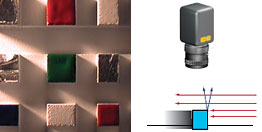
\includegraphics[width=.3\textwidth]{img/illuminazione-tangenziale.jpg}
\caption{Illuminazione tangenziale}\label{fig:illuminazione-tangenziale}
\end{figure}

\begin{centering}
\centering
\begin{tabular}{l l}
Pro: &  Evidenziamento della struttura superficiale dell'oggetto da ispezionare. \\
Contro: &  Punti lumininosi ed eccessiva generazione di ombre \\
\end{tabular}
\end{centering}


\subsection{Illuminazione diffusa}
Un illuminatore tangenziale è costituito da sorgente di luce 
diffusa ed estesa ciò li rende adatti nell’ispezione di parti 
che potrebbero creare riflessi illuminando in maniera 
omogenea e consistente l’area di ispezione, sono tuttav ia 
di difficile impiego in contesti dove gli ingombri sono 
ridotti per via delle grandi dimensioni ( Una sorgente di 
luce diffusa viene realizzata posizionando sorgenti di luce 
puntiforme lontano dall’area di ispezione )  
 

\begin{figure}
\centering
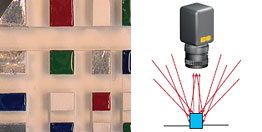
\includegraphics[width=.3\textwidth]{img/illuminazione-diffusa.jpg}
\caption{Illuminazione diffusa}\label{fig:illuminazione-diffusa}
\end{figure}


\begin{centering}
\centering
\begin{tabular}{l l}
Pro: &  Riduce al minimo i riflessi e provvede ad un illuminazione uniforme. \\
Contro: &  Grandi dimensioni, difficoltà di realizzazione \\
\end{tabular}
\end{centering}

\subsection{Illuminazione anulare}
Un illuminatore anulare è costituito da più sorgenti di luce 
puntiformi disposte coassialmente al dispositivo di 
imaging, ciò li rende adatti ad un ispezione simile a quelle 
possibili per mezzo di luce diffusa ma ne limita l’area 
ispezionata e la distanza di esercizio, tale tipologia di 
illuminazione produce inoltre fastidiosi riflessi circolari 
(rumore) 
 


\begin{figure}[h]
\centering
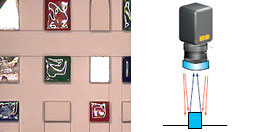
\includegraphics[width=.3\textwidth]{img/illuminazione-anulare.jpg}
\caption{Illuminazione anulare}\label{fig:illuminazione-anulare}
\end{figure}

\begin{centering}
\centering
\begin{tabularx}{\textwidth}{l p{.7\textwidth}}
Pro: &  Il montaggio avviene direttamente sulle lenti, garantisce illuminazione diffusa alla giusta distanza di esercizio. \\
Contro: &  Distanze di impiego limitate, riflessi circolari su superfici riflettenti.\\
\end{tabularx}
\end{centering}

\subsection{Illuminazione diffusa assiale}
Un illuminatore diffuso assiale  è costituito da una 
sorgente di luce puntiforme direzionale orientata 
perpendicolarmente all’oggetto da ispezionare, tale luce 
colpisce un beam splitter riflettendosi prima sulla parte da 
ispezionare e poi sul dispositivo di imagin, ciò crea una 
luce diffusa senza riflessi circolari ma gli  ingombri di 
questi sistemi e la distanza di esercizio limitata ne 
vincolano l’utilizzo 
\begin{figure}[!h]
\centering
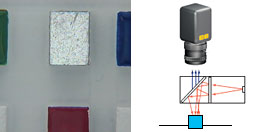
\includegraphics[width=.3\textwidth]{img/illuminazione-diffusa-assiale.jpg}
\caption{Illuminazione diffusa assiale}\label{fig:illuminazione-diffusa-assiale}
\end{figure}



\begin{centering}

\begin{tabular}{l l}
Pro: &  Illuminazione uniforme, riduzione delle ombre, pochi riflessi \\
Contro: &  Dimensioni elevate, difficile montaggio, bassa efficienza.\\
\end{tabular}
\end{centering}


\subsection{Illuminazione strutturata}
Un illuminatore a luce strutturata è costituito da una sorgente che proietta
pattern geometrici quali, linee, punti, griglie o cerchi, tale struttura della
luce può evidenziare curvature o altri difetti dei materiali o essere utile 
per effettuare misure basate sulla distorsione dei motivi proiettati.

\begin{figure}[!h]
\centering
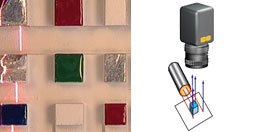
\includegraphics[width=.3\textwidth]{img/illuminazione-strutturata.jpg}
\caption{Illuminazione strutturata}\label{fig:illuminazione-strutturata}
\end{figure}



\begin{centering}

\begin{tabularx}{\textwidth}{l p{.8\textwidth}}
Pro: &  Genera un elevata luminosità su piccole arre di interesse, possibilità di misurare la profondità.\\
Contro: &  Può causare riflessi ed è assorbita da alcuni colori.\\
\end{tabularx}
\end{centering}

\subsection{Illuminazione polarizzata}
Un illuminatore polarizzato è costituito da una sorgente di luce polarizzata e di
un analizzatore (montato sul sensore), ciò permette di eliminare selettivamente
riflessi provenienti da specifiche direzioni.

\begin{figure}[!h]
\centering
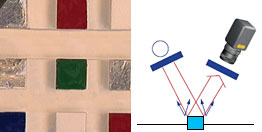
\includegraphics[width=.3\textwidth]{img/illuminazione-polarizzata.jpg}
\caption{Illuminazione polarizzata}\label{fig:illuminazione-polarizzata}
\end{figure}

\begin{centering}

\begin{tabular}{l l}
Pro: &  Genera una superfice con illuminazione uniforme e con riflessi ridotti.\\
Contro: &  Diminuisce l'efficienza del sistema di illuminazione.\\
\end{tabular}
\end{centering}

\subsection{Illuminazione dark-field}
Un illuminatore dark-field è costituito da una sorgente direzionale di luce posizionata perpendicolarmente
alla lente, la luce penetra così un oggetto traslucente attraverso i bordi

\begin{figure}[!h]
\centering
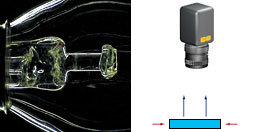
\includegraphics[width=.3\textwidth]{img/illuminazione-darkfield.jpg}
\caption{Illuminazione dark-field}\label{fig:illuminazione-darkfield}
\end{figure}

\begin{centering}

\begin{tabularx}{\textwidth}{l p{.8\textwidth}}
Pro: &  Altissimo contrasto sui dettagli interni e superficiali. esalta graffi crepe e bolle in oggetti trasparenti \\
Contro: &  Basso contrasto sui bordi, non funziona su oggetti opachi.\\
\end{tabularx}
\end{centering}

\subsection{Retroilluminazione (bright-field).}
Un illuminatore bright-field è costituito da una sorgente di luce posta sul retro dell'oggetto da ispezionare,
ciò può essere utile per evidenziarne i contorni a scopo di misura o per osservare dettagli in un oggetto
trasparente 

\begin{figure}[!h]
\centering
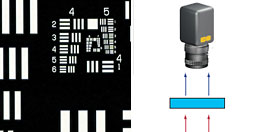
\includegraphics[width=.3\textwidth]{img/illuminazione-brightfield.jpg}
\caption{Illuminazione brightfield}\label{fig:illuminazione-brightfield}
\end{figure}

\begin{centering}

\begin{tabularx}{\textwidth}{l p{.8\textwidth}}
Pro: &  Alto contrasto per il rilevamento dei bordi. \\
Contro: &  Elimina i dettagli superficiali.\\
\end{tabularx}
\end{centering}

